%%%%%%%%%%%%%%%%%%%%%%%%%%%%%%%%%%%%%%%%%%%%%%%%%%%%%%%%%%%%%%%%%%%
%                                                                 %
%   KUIP  - Reference Manual -- LaTeX Source                      %
%                                                                 %
%   Chapter 1: User Interface Management Systems and KUIP         %
%                                                                 %
%   External EPS files referenced: lay.eps, layer.eps             %
%                                                                 %
%   Editor: Michel Goossens / CN-AS                               %
%   Last Mod.: 10 Dec  1992   mg                                  %
%                                                                 %
%%%%%%%%%%%%%%%%%%%%%%%%%%%%%%%%%%%%%%%%%%%%%%%%%%%%%%%%%%%%%%%%%%%

\chapter{User Interface Management Systems and \KUIP{}}
 
\KUIP{} (Kit for a User Interface Package) is the User
Interface system developed at CERN in the context of \PAW{},
the Physics Analysis Workstation system \cite{bib-PAW,bib-PAWART}.

\begin{figure}[tb]
\begin{center}
\mbox{\epsfig{file=lay.eps,width=\textwidth}}
\end{center}
\vspace{-.5cm} 
\caption{The homogeneous environment provided by a U.I.M.S.}
\label{FIG1}
\end{figure}

A User Interface Management System (UIMS) is a software toolkit intended to:
\begin{ULc}
\item
provide a homogeneous environment in which different kinds of
\textbf{users}
interact with different kinds of applications (see Figure~\ref{FIG1}).
\item
provide tools to help the programmer in developing an interactive
application.
\end{ULc}

Each application usually has a heterogeneous user base at different
levels of experience. 
The design of a UIMS should aim at a good compromise between the ease
of use for beginners and the avoidance of frustration for more experienced
users.
A beginner or casual user may prefer a menu mode for guiding him
through the set of command, while a user who is already familiar with
an application can often work more efficiently with a command line mode.

Both requirements can only be met by a 
\textbf{multi-modal dialogue}
system, i.e.\ the application has to provide different dialogue
styles with the possibility to switch between them from inside the
application. 
In any case the UIMS should allow to include enough 
\textbf{online-help}
to make the application usable without any additional written documentation.

Another important point is to allow 
\textbf{mixed control}
of command execution.
In the usual case the command processor prompts the user for the next
command and passes it onto the application.
On the other hand the application should also be able to pass command
sequences back to the command processor for execution.

%
%---------------------------------------------------------------------------
%
\section{The Layers of \KUIP{}}

As a User Interface system \KUIP{} concerns both the application
writer and the application user.
Figure~\ref{FIG2} shows the different layers in a \KUIP{}-based application.
The ordinary user only has to know about the top layer with standard
rules how to select a command and how to supply the necessary arguments.

\begin{figure}[tb]
\begin{center}
\mbox{\epsfig{file=layer.eps,height=12cm}}
\end{center}
\caption{The different layers in a \KUIP{} application}
\label{FIG2}
\end{figure}

The application writer on the other hand has to understand the tools
which allow to define the command structure for the middle layer.
He also has to provide the bottom layer which implements the specific code
for each command.

%
%---------------------------------------------------------------------------
%
\subsection{The Application Writer's View}

The application writer has to describe the command tree structure and
the parameters and action routines associated with each command.
In order to do its job \KUIP{} has to store this information in
internal structures.
The possibility that the application programmer has to write himself
the routine calling the appropriate \KUIP{} routines was considered as
being too inconvenient.

Instead the application writer only has to provide a text file
called the Command Definition File~(\CDF{}) containing a formal
description of the command set.
A stand-alone program, the
\KUIP{} Compiler (\KUIPC{}),
analyzes the \CDF{} and generates a file containing the source code
(i.e.\ calls to \KUIP{} routines) to store the
command structure at run-time.

The routine generated by \KUIPC{} has to be called by the
application program once between the initialization of \KUIP{}
(\Rind{KUINIT}) and the point when control is passed to the 
\KUIP{} main input loop (\Rind{KUWHAT}).
For the commands given by the user \KUIP{} calls the associated 
action routines which have to be provided by the application writer.
The action routine can then retrieve the command arguments
(\KUGETx{}) and perform the appropriate actions.
The \CDF{} allows to specify parameters as being mandatory (for which the user
must supply an argument value) or optional (for which the \KUGETx{}
routines return a default value if omitted by the user).

Generating the actual command definition code automatically from the
higher-level \CDF{} format offers many advantages:
\begin{UL}
\item
The directives needed to mark-up the \CDF{} description are easier to
learn than the calling sequences and correct ordering of the
definition routines.
\item
The command structure is better visible in the \CDF{} than in the
corresponding source code cluttered by calls to cryptic routine
names with cryptic option arguments. 
\item
The \CDF{} is far easier to edit because the writer does not have to
worry about continuation lines or the correct quoting of character
strings.
\item
\KUIPC{} gives the choice between generating C or Fortran source code.
Using the C~output mode can considerably reduce an application's
start-up time.
\KUIPC{} can allocate most of the structures statically that building
the command tree involves only a few pointer manipulations.
On the other hand the Fortran output mode allows to keep the installation
procedures simple for otherwise purely Fortran-based applications.
\end{UL}
%
%---------------------------------------------------------------------------
%
\subsection{The Application User's View}

\KUIP{} provides different dialogue modes (or styles) how the user can
enter commands:
the default command line input from the keyboard and
various menu modes either driven by keyboard input or by mouse clicks.
Switching between dialogue styles is possible at any moment
during the interactive session.
This makes \KUIP{} suitable to applications with a heterogeneous user
base:
each user can choose according to his taste and knowledge of the
application.

In command line mode \KUIP{} writes out a prompt and waits for input
from the user. 
The input consists of a command name possibly followed by an argument
list.
The command name can be abbreviated and \KUIP{} matches it
against the set of defined commands.
Then the arguments given on the input line are
assigned to the command parameters.
If any of the mandatory arguments is missing the user is prompted to
enter a value for them.
If a character string appears in a position where a number is expected
or if a numeric value is outside the allowed range the user is
prompted again to correct the argument.
Only when the input passes these basic consistency checks \KUIP{}
calls the action routine and issues the next command line prompt.
 
%-------------------------------------------------------------------------
\section{A Quick Look at the Main Features of \KUIP{}}

\KUIP{} represents a general-purpose User Interface Management Systems.
The basis of \KUIP{} is the so-called
Command Definition File~(\CDF{}) containing a description of the command
parameters, on-line help information, and how the commands are grouped
into menus.
Since menus can be linked to other menus the application commands are
represented by an inverted tree in analogy to a Unix file system. 
The \KUIP{} Compiler (\KUIPC{}) converts the \CDF{} into routines which
have to be compiled and linked with the interactive application.

The interaction between the user and the application is either
by typing command lines or selecting command from alphanumeric or
graphical menus. 
The user is able to switch between dialogue modes at any time.
In menu mode the user can traverse the command tree and select commands
for execution.
This does not require any additional programming from the application
writer since the menu structure is already described in the \CDF{}.

The commands typed-in may be abbreviated by omitting parts of the
complete command path as long as this does not produce ambiguities
between different commands.
Previous command lines can be recalled, edited, and re-executed.
A \texttt{csh}-like history mechanism is also available.

\KUIP{} provides a macro language with variables, expressions, and
various control flow constructs which allows to execute a complex
sequence of commands by typing a single \Cind{EXEC} command.
An application can execute a logon macro at start-up time that the
user can configure the environment to his taste.
All command lines entered during a sessions are recorded in form of a
macro file which can be the starting point for a proper macro.
An application can also be run in batch mode by executing a macro file
without any user interaction.

The documentation for each command is contained inside the \CDF{}.
Keeping the \CDF{} up-to-date guarantees that the on-line help derived
from it is always in phase with the actual program version.
\KUIP{} allows to write out the command description marked-up with
\LaTeX{} formatting command which then can be included in the proper
users' guide or reference manual.

 
\section{The Advantages of Using \KUIPMotif{}}

\Motif{} \cite{bib-MOTIF} is a widget set developed by the Open
Software Foundation (OSF).
Most major computer vendors joined OSF and support \Motif{} as part of their
system software.

\KUIPMotif{} is an extension to the basic \KUIP{} package which
interfaces to the \Motif{} windowing system.
Again, the development of \KUIPMotif{} started off in the context of
\PAW{}.
The aim was to generalize the ideas which went into the \Motif{}
version \PAW++{} and make them available to other, already
existing \KUIP{}-based applications.

As a result an application programmer can supply his users a powerful
windowing interface with minimum effort.
By merely changing a few \KUIP{} initialization calls the application
inherits already most of the \KUIPMotif{} functionalities 
(see figures~\ref{ref:FIGPKMF1} and~\ref{ref:FIGPKMF2}):
\condbreak{3\baselineskip}
\begin{UL}
\item
A terminal window allows to type commands and to scroll through the
application output messages.
\item
A general object browser visualizes the command tree and file system
structure.
The browser window can be ``cloned'' to look at different parts of the
object trees at the same time.
Commands can be invoked by browsing through the command tree or from
pull-down menus attached to the browser window.
Arguments can be filled into command panels showing the completely list
of command parameters and option values.
\item
User defined panels allow to execute command sequences by a single
mouse click.
\item
\KUIPMotif{} cooperates with \HIGZ{}/X11 and allows for
several simultaneous graphics windows.
\end{UL}

In order to take full advantage of the \KUIPMotif{} facilities the
application writer has to spend only a little more effort.
The central point of \KUIPMotif{} is the object browser.
Every application deals with some kind of ``objects'' which are often
linked into a hierarchical tree structure.
The \KUIPMotif{} browser allows the user to traverse and visualize the
content of the tree and to operate on individual objects.

The actual nature of these ``objects'' is arbitrary.
For example, in \PAW{} the prime objects are histograms and N-tuples,
while in \GEANT{} they are the volumes in the detector geometry or the
particle tracks in an event simulation.
Application-specific objects are integrated into the browser defining
the possible objects types in the \CDF{}.
The only additional coding work required is to provide a routine
which, given the path selected in the browser window, scans the
directory content and returns for each object its identification
(section \ref{ref:rebrodef}).

An object is identified by its name and its type.
The type names or ``classes'' are defined in the \CDF{} and determine
the icon used for showing the object and the list of possible actions
to operate on a selected object.
The value returned as object ``name'' is up to the
scanning routine but naturally it should be the same usually required
to refer to the object in a command.
Behind the class-specific action menus there are command sequences
which allow to insert the object name in the appropriate position.
If the object name is the only item necessary to make the command
complete it can be executed immediately, otherwise the command
panel pops up where the user can enter the missing arguments. 

One of the main advantages of \KUIPMotif{} is that all applications
will give the users the same ``look and fill''.
Further design goals met by \KUIPMotif{} are:
\begin{UL}
\item
\KUIPMotif{} can be used without any prior knowledge about \Motif{}
programming.
On the other hand \KUIPMotif{} provides the hooks to integrate
application specific \Motif{} widgets into the user interface.
\item
For an existing \KUIP{} based application a \Motif{} interface can be
provided by changing of a few initialization calls only.
\item
In order to exploit to the full power of \KUIPMotif{} the application
writer has to add new routines rather than to change existing ones.
Therefore the whole application code can reside in a single library,
while the different initialization calls between basic \KUIP{} and
\KUIPMotif{} can be absorbed in the main program.
\item
For convenience a single module can contain both the basic \KUIP{} command
line interface and the \KUIPMotif{} interface giving the user the
choice at startup time.
Loading the \Motif{} libraries adds typically 2--3~Mbytes to the module size.
If memory is at a premium a module with the basic \KUIP{} command line
can be generated which does not required any \Motif{} specific code to
be loaded.
\item
Although \KUIPMotif{} is fully integrated with the \HIGZ{}/X11
graphics package a non-graphical application does not need to load any
\HIGZ{} code.
\end{UL}

%
%---------------------------------------------------------------------------
%
\section{Implementation and Portability}

Originally \KUIP{} was written at CERN completely in Fortran~77.
The choice of Fortran as implementation language was governed by the
fact that at that time~(1987) the Fortran compiler was the only one commonly
available on all initial target platforms (VM/CMS, VAX/VMS, and Apollo).
However, Fortran misses a number of language features which are
essential for programming a User Interface package:
recursivity, function pointers, and recovery from exceptions.

Already with the advent of Unix workstations
some system dependent tasks could not be expressed in Fortran
anymore and had to be written in C.
The use of \KUIP{} in various applications with widely different
requirements made evident another limitation of Fortran:
The purely static allocation of character variables leads to a
trade-off between wasted memory space and the risk that one
application could still need more than the fixed size limit.

For the \KUIP{} version released in the beginning of 1992 major parts
were rewritten in~C.
The rewrite removed most of the size limitations, added new
functionalities, and at the same time improved the portability by placing
non-standard Fortran with standard C constructs.
Storing the command tree in C~structures also simplified the
implementation of the \Motif{} interface (which was written in~C from the
very beginning) considerably because it obsoleted routines previously
needed for accessing the information stored inside \ZEBRA{}
structures.

Two main parts of \KUIP{} are still mainly in Fortran: the handling of
vectors and the macro compiler/interpreter.
Both have a number of limitations which can be avoided using~C.
The intention is to replace them by C~code as well, and at the same
time formalize the interface for using \KUIP{} directly from applications
written in~C.

\KUIP{} is part of the CERN \PACKLIB{} and partially depends on other
standard packages included in this library.
Several large CERN application programs use \KUIP{}:
\PAW{}\cite{bib-PAW}, \GEANT{}\cite{bib-GEANT}, and \CMZ{}\cite{bib-CMZ} 
amongst others.
The basic \KUIP{} has also been ported to the following
vendor/operation systems where underlining indicates the platforms for
which ready-to-use libraries are available from the CERN program library:
\begin{DL}{1234567}
\item[Convex:]
Convex-OS
\item[Cray:]
Unicos
\item[DEC:]
\underline{\vphantom{p}Vax/VMS},
\underline{\vphantom{p}RISC/Ultrix}, 
Vax/Ultrix,
\underline{Alpha/VMS},
\underline{Alpha/OSF}, 
Alpha/Windows-NT
\item[HP:]
\underline{Apollo/Domain-OS},
\underline{\vphantom{p}HP/UX}
\item[IBM:]
\underline{\vphantom{p}VM/CMS}, 
MVS/TSO, 
NEWLIB (DESY MVS),
\underline{\vphantom{p}RS-6000/AIX}
\item[SGI:]
\underline{\vphantom{p}Irix}
\item[Sun:]
\underline{\vphantom{p}Sun-OS}, 
\underline{\vphantom{p}Solaris}
\item[PC:]
MS-DOS, 
NeXT,
\underline{\vphantom{p}Linux}
\end{DL}

\condbreak{5\baselineskip}
\KUIPMotif{} requires the \Motif{} libraries version~1.1 or later.
It is known to be working on the following platforms:
\begin{DL}{12345}
\item[DEC:]
\underline{\vphantom{p}RISC/Ultrix V4.3}, 
\underline{\vphantom{p}Vax/VMS},
\underline{Alpha/VMS},
\underline{Alpha/OSF}
\item[HP:]
\underline{Apollo/Domain-OS SR10.4} (not for DN10000),
\underline{\vphantom{p}HP/UX}
\item[IBM:]
\underline{\vphantom{p}RS-6000/AIX}
\item[SGI:]
\underline{\vphantom{p}Irix}
\item[Sun:]
\underline{\vphantom{p}Sun-OS} 
(with DEC-Motif libraries and using the DEC-Motif window manager),
\underline{\vphantom{p}Solaris} 
\end{DL}



